\documentclass{article}

\usepackage{amssymb}
\usepackage{mathtools}
\usepackage{algorithm}
\usepackage[noend]{algpseudocode}
\usepackage{biblatex}

\addbibresource{ref.bib}

\begin{document}

\section{Monte Carlo Integration}

\subsection{Primary-Sample-Space Formulation}

We want to use the technique of Monte Carlo to estimate the integration formulation of the light transport problem. The light transport problem is formulated as follows. Our problem is formulated from an implementation perspective that is much easier to understand. Consider the function $L$ that gives the radiance of a light path. See how we map a light path to the radiance.

We define a light path over a so-called primary sample space with infinite dimensions. Notice how tracing a ray involves choosing a random number and decide on a direction. The formulation is motivated from an implementation perspective. When tracing a light path in a path tracer, we first need the pixel position on the camera we are tracing, and then we determine the initial ray direction. At each surface scattering event, we need to determine a scattering direction that is still done by choosing a random numbers. To emulate the fuzziness on the mirror, a small perturbation vector is added to the reflection direction. Throughout the implementation, we can observe that random numbers are widely used and that a sequence of random numbers uniquely determines the light path.

Therefore, in our formulation, a light path is uniquely determined by a vector $\vec{x}$ over $[0, 1]^\infty$ that can be considered as a sequence of random numbers over $[0, 1]$. Given this formulation, we can map any vector of infinite dimensions to a light path and compute its radiance using the function $L$. For the $i$th pixel, spectrum of the light is given by the following integration:
\[
    I_i = \int h_i(\vec{x})\vec{L}(\vec{x})d\vec{x},
\]
    where $h_i(\vec{x})$ is an indicator function that is zero if $\vec{x}$ doesn't correspond to the $i$th pixel.

To estimate the integration value, we use a technique called Monte-Carlo. Given N samples $X_1, X_2, \dots, X_N$ drawn from the distribution $p$, the integration above can be estimated by
\[
    \frac{1}{N}\sum_{k = 1}^N \frac{f(X_k)}{p(X_k)}.
\]
This can be easily verified by the law of large numbers, as the expected value of each term in the summation is
\[
    E\left[\frac{f(X_k)}{p(X_k)}\right] = \int \frac{f(x)}{p(x)}p(x)dx = \int f(x)dx.
\]

Therefore, to compute the value for each pixel on the image, we just need to sample a number of random variables, map them to light paths and accumulate the spectrum values.

\subsection{Metropolis Light Transport}

We introduce the primary-sample-space Metropolis light transport (PSSMLT) algorithm \cite{pbrt}. This formulation is different from the original Metropolis light transport algorithm that is prone to implementation errors. The core idea of PSSMLT is to control the distribution of the samples $p$ used in Monte Carlo integration so that $p$ is proportional to $L$. In this way, paths contributing more light will be heavily sampled while paths contributing less light will be lightly sampled.

Note that the proof of correctness for Monte Carlo integration shows that regardless of the distribution used for sampling, the estimated value converges to the true value as the number of samples approaches infinity. The major benefit is better rendering quality and faster convergence.

The remaining problem is how to sample from a distribution proportional to $L$. The solution is to use the Metropolis-Hasting algorithm. The algorithm allows sampling from a distribution that is proportional to given function $f(x)$ with the condition being that $f(x)$ can be evaluated. That is, it can generate samples from the normalized distribution
\[
    p(x) = \frac{f(x)}{\int f(x)dx}
\]
as long as $f(x)$ can be evaluated.

Let $f(x)$ be a function that can be evaluated for any $x$ and returns a scalar. Metropolis algorithm generates a series of samples $x_1, x_2, \dots, x_N$ from a distribution whose probability density is proportional to $f(x)$ based on an initial value $x_0$. Given a sample $x_i$, the algorithm applies a mutation to $x_i$ to generate a \emph{tentative sample} $x_{i + 1}'$. The tentative sample is accepted with probability $a(x_{i + 1}'|x_i)$. When the sample is accepted, we set $x_{i + 1}$ to $x_{i + 1}'$. If the sample is rejected, $x_{i + 1}$ is still $x_i$.

To set the acceptance probability, suppose we already manage to sample $x_{i + 1}$ from our target distribution $p(x)$. Let $p_i$ be the distribution from which sample $x_i$ is drawn, we have
\begin{equation}
    \label{eq:sample-cdf}
    p_{i + 1}(x) = \int K(x|y)p_i(y)dy
\end{equation}
where $K(x|y)$ is the \emph{transition probability} from $y$ to $x$ and is
\[
    K(y|x) = a(y|x)T(y|x)
\]
with $K(x|x) = 1$ and $T$ being the tentative transition probability that characterizes the probability of generating $y$ by mutating $x$.

When the tentative transition probability and acceptance probability satisfies the following \emph{detailed balance condition}
\[
    a(y|x)T(y|x)f(x) = a(x|y)T(x|y)f(y)
\]
we have $p_{i + 1} = p$. To verify this, replace $K$ with $a$ and $T$ in Equation~(\ref{eq:sample-cdf}):
\begin{align*}
    p_{i + 1}(x) &= \int a(x|y)T(x|y)p_i(y)dy + \left[1 - \int a(y|x)T(y|x)dy\right]p_i(x)\\
    &= p_i(x) = p(x)
\end{align*}

The detailed balance condition is intuitive for a physical system. In a physical system, the probability of choosing $x$, mutating $x$ and generating $y$ should be equal to the probability of its reverse: choosing $y$ and generating $x$. The physical system is said to reach equilibrium.

In order to reach equilibrium as quickly as possible, the best strategy is to make the acceptance probability as large as possible, which is achieved by setting
\[
    a(y|x) = \min\left(1, \frac{T(x|y)f(y)}{T(y|x)f(x)}\right).
\]
According to this rule, transitions in one direction are always allowed, while in the other direction is sometimes allowed.

Other details about the algorithm are included below:

\begin{description}
    \item[Mutation strategies] Two mutation strategies are used in PSSMLT: a small-step mutation that adds a random perturbation from a normal distribution to each dimension of the current sample, and a large-step mutation that regenerates a new light path from a uniform distribution. The tentative transition probability for these strategies is symmetric i.e., $T(y|x) = T(x|y)$, which means the acceptance probability only depends on the target distribution.
    \item[Spectrum-to-probability function] Because the integrand $\vec{L}$ returns a vector for spectrum that can't be used directly as probability, we compute the luminance $s$ of a spectrum and use it as the target distribution for Metropolis sampling. The complete formula for computing the value $I_i$ for pixel $i$ is
    \[
        I_i = \frac{b}{N}\sum_{j = 1}^N h_i(x_j) \frac{\vec{L}(x_j)}{s[\vec{L}(x_j)]}
    \]
    and $b$ is the normalization term $b = \int s[\vec{L}(x)]dx$.

    \item[Bootstrapping] The bootstrapping step helps to solve two problems in the implementation of the Metropolis algorithm: how to compute the normalization term $b$ and how to select the initial value $x_0$. The method used is to first choose a set of paths and then sample the initial value from this set of sample paths. The normalization term is also estimated from this set of paths.
    
    \item[Expected-value technique] One problem with MLT is that when a tentative sample is proposed and then rejected, all computation associated with it is effectively ``wasted'' because the computed spectrum isn't added to the final image. A technique \cite{mlt} is proposed that adds tentative samples to pixel value, even if it's rejected.
\end{description}

The PSSMLT algorithm is shown in Algorithm~\ref{alg:pssmlt}.

\begin{algorithm}
    \caption{PSSMLT}
    \label{alg:pssmlt}
    \begin{algorithmic}[1]
        \For{$i \gets 1$ \textbf{to} $N$}
            \State Mutate $x_{i - 1}$ to generate the tentative sample $x_i'$.
            \State Record $x_{i - 1}$ and $x_i'$ in the image.
            \State $a \gets \min\{1, s[\vec{L}(x_i')] / s[\vec{L}(x_{i - 1})]\}$
            \State Roll a dice to determines whether to accept or reject.
            \If{Accept}
                \State $x_i \gets x_i'$
            \Else
                \State $x_i \gets x_{i - 1}$
            \EndIf
        \EndFor
    \end{algorithmic}
\end{algorithm}

\section{Evaluation}

To compare the effectiveness of Monte-Carlo integration and PSSMLT, we render a modified Cornell box scene that contains a glossy metal box and a glass ball with a resolution of $100 \times 100$. The rendered images are shown in Figure~\ref{fig:monte-carlo}. The rendering shows that PSSMLT is good at rendering the reflection of light by the glass ball without bright noises all over the image. The better quality of reflection is likely the result of PSSMLT's small-step mutation, where local paths with for the reflection are thoroughly explored. On the other hand, PSSMLT's rendering of the scene is fuzzier and less uniform on direct illumination e.g., walls in the scene.

\begin{figure}
    \centering
    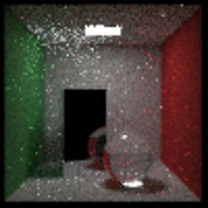
\includegraphics{monte-carlo.pdf}
    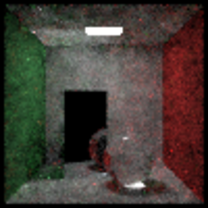
\includegraphics{pssmlt.pdf}
    \caption{Comparison of Monte-Carlo integration and PSSMLT in a modified Cornell box scene. The image on the right is produced by PSSMLT.}
    \label{fig:monte-carlo}
\end{figure}

% what's still missing? evaluation, evaluation, evaluation, evaluation.

\printbibliography

\end{document}
